\documentclass[a4paper, 12pt]{article}
\usepackage[utf8]{inputenc}
\usepackage[brazil]{babel}
\usepackage[top=2cm, bottom=2cm, left=3cm, right=2cm]{geometry}
\usepackage{indentfirst}
\usepackage{graphicx}
\usepackage{amsmath}
\usepackage{physics}
\usepackage{float}
\usepackage{multirow}

\newtheorem{teo}{Teorema}[subsection]
\newtheorem{defi}{Definição}[section]

\newcommand{\divfield}[1]{\div{\textbf{#1}}}
\newcommand{\curlfield}[1]{\curl{\textbf{#1}}}

\begin{document}

\begin{center}
    \Large UNIVERSIDADE FEDERAL DE SERGPE\\CENTRO DE CIÊNCIAS EXATAS E DA TERRA\\DEPARTAMENTO DE FÍSICA
    
    \vspace{50mm}
    
    \normalsize
    \textbf{Victor S. Nunes}
    
    \vspace{60mm}
    
    \Large
    \textbf{Modelo de TCC escrito em \LaTeX}
    
    \vspace{100mm}
    
    \normalsize
    São Cristóvão, 18 de Agosto de 2021
    
\end{center}
\thispagestyle{empty}

\newpage

\begin{center}
    \Large Victor S Nunes
    \vspace{50mm}
    
    MODELO DE TCC ESCRITO EM \LaTeX
\end{center}
\vspace{50mm}

\begin{flushright}
Trabalho de Conclusão de Curso submetido à\\Universidade Federal de Sergipe como requisito\\para receber o grau de bacharel em Astrofísica
\end{flushright}
\vspace{95mm}

\begin{center}
    \normalsize
    São Cristóvão, 18 de Agosto de 2021
\end{center}
\thispagestyle{empty}

\newpage
\abstract{Lorem ipsum dolor sit amet, consectetur adipiscing elit. Aliquam vitae feugiat ex, nec condimentum tortor. Aliquam vulputate odio eget dictum mollis. Nam dictum, felis in tempor placerat, nibh diam mollis risus, et volutpat ante magna a sapien. Vivamus aliquet tristique augue ac semper. Nulla pretium felis et lectus lobortis aliquam. Quisque aliquet sapien a leo posuere molestie in a felis. Aenean hendrerit urna eu vestibulum pretium. Morbi id quam vitae ligula placerat fermentum. Fusce eget maximus metus, sed rhoncus ligula. Ut pellentesque, quam et iaculis ornare, tortor libero finibus purus, quis convallis sem tortor ut metus. Praesent tempus neque id velit ornare porttitor. Pellentesque eleifend nec dui ac imperdiet. Sed dapibus, odio non laoreet ultricies, eros lectus aliquet quam, euismod gravida purus dolor eget nisl. Cras ut erat a nunc eleifend lobortis dictum id lorem. Donec consectetur ullamcorper risus vitae porttitor. Interdum et malesuada fames ac ante ipsum primis in faucibus.}
\thispagestyle{empty}

\newpage

\listoffigures
\thispagestyle{empty}
\newpage

\listoftables
\thispagestyle{empty}
\newpage

\tableofcontents
\thispagestyle{empty}

\setcounter{page}{0}
\newpage

\section{Introdução}
Lorem ipsum dolor sit amet, consectetur adipiscing elit. Aliquam vitae feugiat ex, nec condimentum tortor. Aliquam vulputate odio eget dictum mollis. Nam dictum, felis in tempor placerat, nibh diam mollis risus, et volutpat ante magna a sapien. Vivamus aliquet tristique augue ac semper. Nulla pretium felis et lectus lobortis aliquam. Quisque aliquet sapien a leo posuere molestie in a felis. Aenean hendrerit urna eu vestibulum pretium. Morbi id quam vitae ligula placerat fermentum. Fusce eget maximus metus, sed rhoncus ligula. Ut pellentesque, quam et iaculis ornare, tortor libero finibus purus, quis convallis sem tortor ut metus. Praesent tempus neque id velit ornare porttitor. Pellentesque eleifend nec dui ac imperdiet. Sed dapibus, odio non laoreet ultricies, eros lectus aliquet quam, euismod gravida purus dolor eget nisl. Cras ut erat a nunc eleifend lobortis dictum id lorem. Donec consectetur ullamcorper risus vitae porttitor. Interdum et malesuada fames ac ante ipsum primis in faucibus.

Morbi interdum commodo est, vel egestas lacus vulputate quis. Sed eu justo bibendum, accumsan elit eget, posuere nibh. Nunc auctor lorem ante, in scelerisque est tincidunt at. Mauris eget arcu luctus enim accumsan condimentum. Morbi ullamcorper risus sed scelerisque volutpat. Integer pretium auctor ante at congue. Aenean tristique, lorem in sodales tincidunt, leo magna fringilla nulla, ut molestie diam nisl vel velit. Nullam imperdiet sapien at suscipit vulputate. Phasellus bibendum ultrices ligula, ac sollicitudin nulla. Interdum et malesuada fames ac ante ipsum primis in faucibus. Sed maximus ipsum eget justo cursus consequat. Quisque nec lorem eget erat vestibulum rhoncus tristique in justo.

\begin{quote}
    Nunc at accumsan nisl. Sed dapibus vel lacus at malesuada. Morbi in odio tempus, pulvinar metus at, sollicitudin dui. Interdum et malesuada fames ac ante ipsum primis in faucibus. Cras cursus, urna et tincidunt varius, elit ligula finibus metus, non laoreet lorem odio vel nibh. Pellentesque pulvinar purus a lacus placerat, a molestie lorem tincidunt. Proin porttitor purus mattis fringilla mollis. Nulla vitae turpis sed urna efficitur egestas ac at nulla. Etiam quis enim neque. Aenean vulputate et lacus id placerat.\footnote{Exemplo de Nota de Rodapé}
\end{quote} Praesent ac nisl at ante condimentum posuere. Vivamus at sagittis mauris. Fusce eget quam elit. Nunc dignissim pharetra dapibus. Mauris id placerat libero, vel molestie sapien.

Phasellus rutrum leo a ornare bibendum. Nam lacus mi, cursus eget cursus non, sodales vel magna. Etiam tristique nisl sed nulla efficitur, at facilisis dui cursus. Vestibulum at feugiat nulla. Nullam feugiat placerat augue vitae faucibus. Nullam feugiat ligula eu massa bibendum imperdiet. Quisque semper ligula erat. Morbi fringilla elit enim, at dictum quam dignissim eu. Sed ac pulvinar felis, quis posuere augue. Maecenas condimentum mollis enim. Mauris elementum maximus ultricies.

\subsection{Problema}
Quisque id mi risus. Integer dignissim purus at nisl ultricies, in porttitor dui iaculis. Duis sed tincidunt libero, et posuere lacus. Sed neque nunc, finibus eget ultricies at, ultricies iaculis turpis. Sed lectus nisl, rhoncus sit amet vestibulum et, egestas id nisi. Fusce ac lacus ac velit faucibus dignissim quis eget ligula. Curabitur blandit nulla vel tempus porttitor. Praesent sed auctor lectus. In fringilla quam a placerat gravida. Vivamus mollis pretium justo dictum vulputate. Proin ullamcorper accumsan odio imperdiet consequat.

\section{Objetivos}
\subsection{Objetivos Gerais}
Lorem ipsum dolor sit amet, consectetur adipiscing elit. Aliquam vitae feugiat ex, nec condimentum tortor. Aliquam vulputate odio eget dictum mollis. Nam dictum, felis in tempor placerat, nibh diam mollis risus, et volutpat ante magna a sapien. Vivamus aliquet tristique augue ac semper. Nulla pretium felis et lectus lobortis aliquam. Quisque aliquet sapien a leo posuere molestie in a felis. Aenean hendrerit urna eu vestibulum pretium. Morbi id quam vitae ligula placerat fermentum. Fusce eget maximus metus, sed rhoncus ligula. Ut pellentesque, quam et iaculis ornare, tortor libero finibus purus, quis convallis sem tortor ut metus. Praesent tempus neque id velit ornare porttitor. Pellentesque eleifend nec dui ac imperdiet. Sed dapibus, odio non laoreet ultricies, eros lectus aliquet quam, euismod gravida purus dolor eget nisl. Cras ut erat a nunc eleifend lobortis dictum id lorem. Donec consectetur ullamcorper risus vitae porttitor. Interdum et malesuada fames ac ante ipsum primis in faucibus.

\subsection{Objetivos Específicos}

\begin{itemize}
    \item Morbi interdum commodo est, vel egestas lacus vulputate quis. Sed eu justo bibendum, accumsan elit eget, posuere nibh. Nunc auctor lorem ante, in scelerisque est tincidunt at. Mauris eget arcu luctus enim accumsan condimentum. 
    \item Morbi interdum commodo est, vel egestas lacus vulputate quis. Sed eu justo bibendum, accumsan elit eget, posuere nibh. Nunc auctor lorem ante, in scelerisque est tincidunt at. Mauris eget arcu luctus enim accumsan condimentum. 
    \item Morbi interdum commodo est, vel egestas lacus vulputate quis. Sed eu justo bibendum, accumsan elit eget, posuere nibh. Nunc auctor lorem ante, in scelerisque est tincidunt at. Mauris eget arcu luctus enim accumsan condimentum. 
     \item Morbi interdum commodo est, vel egestas lacus vulputate quis. Sed eu justo bibendum, accumsan elit eget, posuere nibh. Nunc auctor lorem ante, in scelerisque est tincidunt at. Mauris eget arcu luctus enim accumsan condimentum. 
\end{itemize}

\section{Metodologia}
\begin{enumerate}
    \item Morbi interdum commodo est, vel egestas lacus vulputate quis. Sed eu justo bibendum, accumsan elit eget, posuere nibh. Nunc auctor lorem ante, in scelerisque est tincidunt at. Mauris eget arcu luctus enim accumsan condimentum. 
    \item Morbi interdum commodo est, vel egestas lacus vulputate quis. Sed eu justo bibendum, accumsan elit eget, posuere nibh. Nunc auctor lorem ante, in scelerisque est tincidunt at. Mauris eget arcu luctus enim accumsan condimentum. 
    \item Morbi interdum commodo est, vel egestas lacus vulputate quis. Sed eu justo bibendum, accumsan elit eget, posuere nibh. Nunc auctor lorem ante, in scelerisque est tincidunt at. Mauris eget arcu luctus enim accumsan condimentum. 
    \item Morbi interdum commodo est, vel egestas lacus vulputate quis. Sed eu justo bibendum, accumsan elit eget, posuere nibh. Nunc auctor lorem ante, in scelerisque est tincidunt at. Mauris eget arcu luctus enim accumsan condimentum. 
    \item Morbi interdum commodo est, vel egestas lacus vulputate quis. Sed eu justo bibendum, accumsan elit eget, posuere nibh. Nunc auctor lorem ante, in scelerisque est tincidunt at. Mauris eget arcu luctus enim accumsan condimentum. 
\end{enumerate}

\section{Leis de Maxwell}
Phasellus rutrum leo a ornare bibendum. Nam lacus mi, cursus eget cursus non, sodales vel magna. Etiam tristique nisl sed nulla efficitur, at facilisis dui cursus. Vestibulum at feugiat nulla. Nullam feugiat placerat augue vitae faucibus Figura \ref{maxwell}. Nullam feugiat ligula eu massa bibendum imperdiet. Quisque semper ligula erat. Morbi fringilla elit enim, at dictum quam dignissim eu. Sed ac pulvinar felis, quis posuere augue. Maecenas condimentum mollis enim. Mauris elementum maximus ultricies.

\begin{defi}
Cras cursus, urna et tincidunt varius, elit ligula finibus metus, non laoreet lorem odio vel nibh. Pellentesque pulvinar purus a lacus placerat, a molestie lorem tincidunt. Proin porttitor purus mattis fringilla mollis. Nulla vitae turpis sed urna efficitur egestas ac at nulla.
\end{defi}

\begin{figure}[!htb]
    \centering
    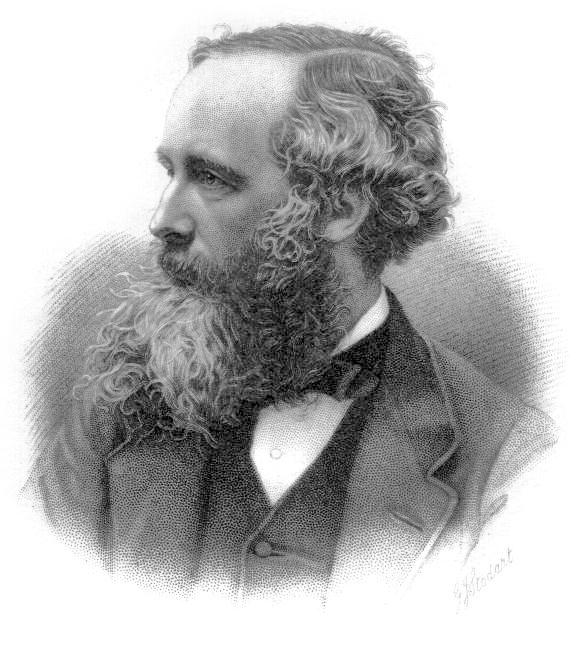
\includegraphics[scale=0.7]{James_Clerk_Maxwell_big.jpg}
    \caption{Maxwell}
    \label{maxwell}
\end{figure}

Etiam quis enim neque. Aenean vulputate et lacus id placerat. Praesent ac nisl at ante condimentum posuere. Vivamus at sagittis mauris. Fusce eget quam elit. Nunc dignissim pharetra dapibus. Mauris id placerat libero, vel molestie sapien.

\begin{description}
    \item[Lei de Gauss] 
                    $$\divfield{E} = \frac{\rho}{\epsilon_{0}}$$
    \item[Lei de Gauss do Magnetismo]
                    $$ \divfield{B} = 0 $$
                    
    \item[Lei de Faraday para Indução]
                    $$\curlfield{E} = -\frac{\partial \textbf{B}}{\partial t}$$
    \item[Lei Circular de Ampère]
                    $$\curlfield{B} = \mu_{0} \left( \textbf{J} + \epsilon_0 \frac{\partial \textbf{E}}{\partial t} \right)$$
\end{description}

\section{Aplicação do Eletromagnetismo}
\subsection{Máquinas Elétricas}
\subsubsection{Transformadores}
Morbi interdum commodo est, vel egestas lacus vulputate quis. Sed eu justo bibendum, accumsan elit eget, posuere nibh. Nunc auctor lorem ante, in scelerisque est tincidunt at. Mauris eget arcu luctus enim accumsan condimentum. Morbi ullamcorper risus sed scelerisque volutpat. Integer pretium auctor ante at congue. Aenean tristique, lorem in sodales tincidunt, leo magna fringilla nulla, ut molestie diam nisl vel velit. Nullam imperdiet sapien at suscipit vulputate. Phasellus bibendum ultrices ligula, ac sollicitudin nulla. Interdum et malesuada fames ac ante ipsum primis in faucibus. Sed maximus ipsum eget justo cursus consequat. Quisque nec lorem eget erat vestibulum rhoncus tristique in justo.

\begin{figure}[!htb]
    \centering
    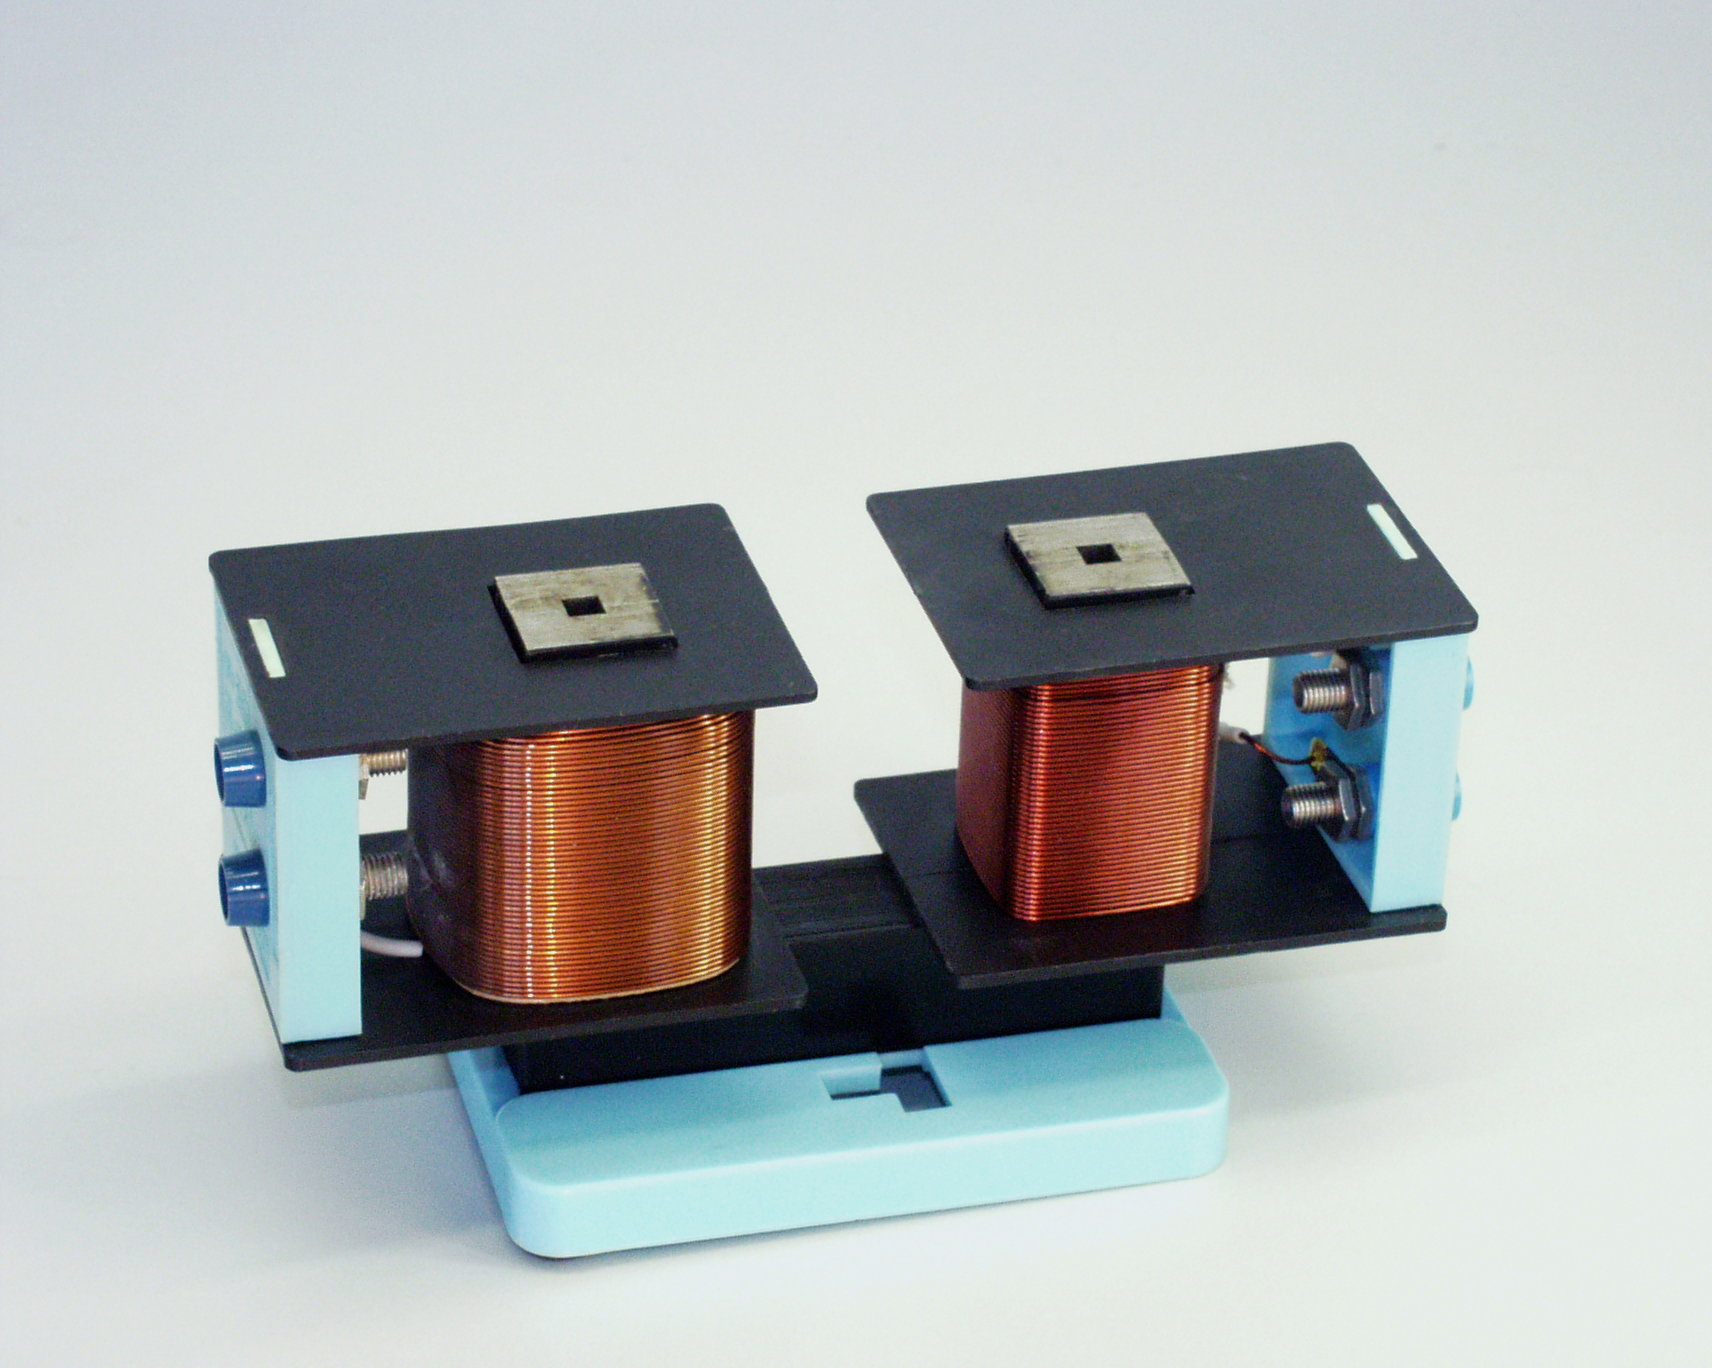
\includegraphics[scale=0.2]{Trafo_3.jpg}
    \caption{Transformador}
    \label{trafo}
\end{figure}

\subsubsection{Motores}
Morbi interdum commodo est, vel egestas lacus vulputate quis. Sed eu justo bibendum, accumsan elit eget, posuere nibh. Nunc auctor lorem ante, in scelerisque est tincidunt at. Mauris eget arcu luctus enim accumsan condimentum. Morbi ullamcorper risus sed scelerisque volutpat. Integer pretium auctor ante at congue. Aenean tristique, lorem in sodales tincidunt, leo magna fringilla nulla, ut molestie diam nisl vel velit. Nullam imperdiet sapien at suscipit vulputate. Phasellus bibendum ultrices ligula, ac sollicitudin nulla. Interdum et malesuada fames ac ante ipsum primis in faucibus. Sed maximus ipsum eget justo cursus consequat. Quisque nec lorem eget erat vestibulum rhoncus tristique in justo.

\section{Resultados}
Morbi interdum commodo est, vel egestas lacus vulputate quis. Sed eu justo bibendum, accumsan elit eget, posuere nibh. Nunc auctor lorem ante, in scelerisque est tincidunt at. Mauris eget arcu luctus enim accumsan condimentum. Morbi ullamcorper risus sed scelerisque volutpat. Integer pretium auctor ante at congue. Aenean tristique, lorem in sodales tincidunt, leo magna fringilla nulla, ut molestie diam nisl vel velit. Nullam imperdiet sapien at suscipit vulputate. Phasellus bibendum ultrices ligula, ac sollicitudin nulla. Interdum et malesuada fames ac ante ipsum primis in faucibus. Sed maximus ipsum eget justo cursus consequat. Quisque nec lorem eget erat vestibulum rhoncus tristique in justo.


\begin{table}[!htb]
\centering
\begin{tabular}{|l|l|c|c|}
\hline
\textbf{Nome}       & \textbf{Localização (ICRS J2000)} & \multicolumn{1}{l|}{\textbf{Banda}} & \multicolumn{1}{l|}{\textbf{Mag}} \\ \hline
PSR B0531+21 (Crab) & 05 34 31.93830 +22 00 52.1758     & V                                   & 16,65                             \\ \hline
PSR B0540-69        & 05 40 10.84 -69 19 54.2           & V                                   & 22,5                              \\ \hline
PSR B0833-45 (Vela) & 08 35 20.65525 -45 10 35.1545     & V                                   & 23,6                              \\ \hline
PSR B0656+14        & 06 59 48.1960 +14 14 19.400       & V                                   & 25                                \\ \hline
Geminga             & 06 33 54.153 +17 46 12.91         & V                                   & 25,5                              \\ \hline
PSR B1055-52        & 10 57 59.0450 -52 26 56.330       & U                                   & 24,9                              \\ \hline
PSR B0950+08        & 09 53 09.2970 +07 55 36.400       & U                                   & 27,1                              \\ \hline
\end{tabular}
\caption{Resultados Experimentais}
\label{resultados}
\end{table}

\nocite{moyses}
\nocite{jackson1999classical}
\nocite{shannon}
\nocite{zero20}
\nocite{sakurai2021modern}

\newpage
\addcontentsline{toc}{section}{Referências}
\bibliographystyle{abbrv}
\bibliography{refs}

\end{document}
